\documentclass[10pt]{article}

\usepackage{amsmath, amssymb, mathtools}
\usepackage{tikz}
\usepackage[margin=1.5cm]{geometry}

\input pdfmsym
\input prettyprint
\input ../preamble

\pdfmsymsetscalefactor{10}
\initpps

\def\pmat#1{\begin{pmatrix} #1 \end{pmatrix}}

\let\divides=\mid
\newfunc{metric}\rho({})
\newfunc{metricc}\sigma({})
\newfunc{ker}{{\rm ker}}({})
\newfunc{spa}{{\rm span}}(\vert)
\newfunc{atan}{{\rm tan}^{-1}}({})
\newfunc{lag}{{\cal L}}({})

\font\bigbf = cmbx12 scaled 2000

\def\openset{{\cal O}}
\let\lineseg=\overleftrightvecc
\let\ds=\displaystyle

\def\pdv#1#2{\frac{\partial #1}{\partial #2}}

\def\differ#1#2{\left.d#1\strut\right|_{#2}}

\def\@ppmathcount{\thesection.\thepp@mathcount}

\def\bexerc{\begin{exercise*}}
\def\eexerc{\end{exercise*}}
\def\bblank{\begin{blankpp}}
\def\eblank{\end{blankpp}}

\begin{document}

\c@section=9

\barcolorbox{220, 255, 220}{0, 130, 0}{80, 200, 80}{
    \leftskip=0pt plus 1fill \rightskip=\leftskip
    {\bigbf Infintesimal Calculus 3}

    \medskip
    \textit{Assignment \thesection}

    \textit{Ari Feiglin}
}

\bigskip

\bexerc
    Find the minimal distance from $(0,0)$ to the hyperbola:
    \[ 7x^2 + 8xy + y^2 = 45 \]
\eexerc

\bblank
    We define the lagrangian:
    \[ \lagof{x,y,\lambda} = x^2 + y^2 + \lambda(7x^2 + 8xy + y^2 - 45) \]
    Whose gradient is
    \[ \pmat{2x + 14\lambda x + 8\lambda y \\ 2y + 2\lambda y + 8\lambda x \\ 7x^2 + 8xy + y^2 - 45} \]
    Solving for zero gives the system
    \[ \pmat{2 + 14\lambda & 8\lambda \\ 8\lambda & 2 + 2\lambda}\cdot\pmat{x\\y} = 0 \]
    So the determinant must be $0$, meaning $\lambda$ is $\frac19$ or $-1$.
    If $\lambda=\frac19$ then this gives us the solution $x=2y$, plugging this into the hyperbola we get $y=\pm1$ and so the point is $\pm(2,1)$.
    $\lambda=1$ gives $y=2x$ and $x=\pm\frac{\sqrt{15}}3$.

    $\pm(2,1)$ gives the minimum distance of $\sqrt5$.
\eblank

\bexerc
    Find the maximum and minimum of the function
    \[ f(x,y,z) = \sqrt2 x + \sqrt2 y + \sqrt3 z \]
    within the ball
    \[ B = \set{(x,y,z)\in\bR^3}[x^2+y^2+z^2\leq2] \]
\eexerc

\bblank
    First we look for critical points within the ball by comparing the gradient of $f$ to $0$, but the gradient of $f$ is
    \[ \nabla f = \pmat{\sqrt2 \\ \sqrt2 \\ \sqrt3} \]
    So we define the lagrangian:
    \[ \lagof{x,y,z,\lambda} = f(x,y,z) + \lambda(x^2+y^2+z^2-2) \]
    And we find critical points relative to it
    \[ \nabla\lag = \pmat{\sqrt2 + 2\lambda x \\ \sqrt2 + 2\lambda y \\ \sqrt3 + 2\lambda z \\ x^2 + y^2 + z^2 - 2} = 0 \]
    So
    \[ x = \frac{\sqrt2}{2\lambda}\quad y = \frac{\sqrt2}{2\lambda}\quad z = \frac{\sqrt3}{2\lambda} \]
    Plugging these into the constraint function we get that
    \[ x^2+y^2+z^2-2 = \frac{7}{4\lambda^2}-2 = 0 \implies \lambda = \pm\frac{\sqrt{14}}4 \]
    And so we have the points $\pm\parens{\frac2{\sqrt7},\frac2{\sqrt7},\sqrt{\frac67}}$, and so the maximum is $\sqrt{14}$ (when the point is positive) and the minimum is $-\sqrt{14}$, as
    the maximum and minimum must be one of these two points.
\eblank

\bexerc
    Find the maximum distance between the origin and the set $\set{(x,y,z)\in\bR^3}[x^2+y^2=1, z=x+y]$.
\eexerc

\bblank
    We are trying to maximize the function $f(x,y,z)=x^2+y^2+z^2$ under the constraints $h_1(x,y,z)=x^2+y^2-1=0$ and $h_2(x,y,z)=x+y-z=0$.
    The Lagrangian of this is:
    \[ \lagof{x,y,z,\lambda_1,\lambda_2} = x^2 + y^2 + z^2 + \lambda_1(x^2+y^2-1) + \lambda_2(x+y-z) \]
    whose gradient is
    \[ \nabla\lag = \pmat{2x + 2\lambda_1x+\lambda_2 \\ 2y + 2\lambda_1y + \lambda_2 \\ 2z - \lambda_2 \\ x^2 + y^2 - 1 \\ x + y - z} \]
    So
    \[ 2x(\lambda_1+1) = -\lambda_2\quad 2y(\lambda_1+1) = -\lambda_2 \quad z = \frac{\lambda_2}2 \]
    If $\lambda_1=-1$ then $\lambda_2=0$ and so $z=0$ and so we're left with $x^2+y^2=1$ and $y=-x$, since there is a solution to this this gives us a distance of $f(x,y,0)=x^2+y^2=1$.

    If $\lambda_1\neq-1$ then
    \[ x,y = -\frac{\lambda_2}{2(\lambda_1+1)} \quad z = \frac{\lambda_2}2 \]
    So $x=y$ and $x^2+y^2=1$ meaning $x^2=\frac12$ so $x=y=\pm\frac1{\sqrt2}$ and $z=x+y=\pm\frac2{\sqrt2}$.
    These are obviously points in the set, so we don't even need to find the values of $\lambda_1$ and $\lambda_2$ since they are inconsequential.
    For these values of $x$, $y$, and $z$ we get
    \[ f(x,y,z) = 1 + z^2 = 3 \]

    So the maximum value of $f$ is $3$ and so the maximum distance is $\sqrt3$.
\eblank

\bexerc
    Compute
    \[ \iiint_D y\,dxdydz \]
    where $D$ is the volume bounded by $y=1-x^2$, $z=0$, and $z=y$.
\eexerc

\bblank
    $D$ can be written as
    \[ D = \set{(x,y,z)\in\bR^3}[0\leq y\leq z,\, y\leq1-x^2] \]
    So $0\leq y\leq 1-x^2$ meaning $-1\leq x\leq 1$, so the integral is equal to
    \[ \int_{-1}^1\int_0^{1-x^2}\int_0^y y\,dzdydx = \int_{-1}^1\int_0^{1-x^2}y^2\,dydx = \frac13\int_{-1}^1(1-x^2)^3\,dx \]
    This is a polynomial, and integrating gives $\frac{32}{105}$.
\eblank

\bexerc
    Reverse the order of integration of
    \[ \int_{-1}^1\int_{x^3}^{\sqrt{2-x^2}} f(x,y)\,dydx \]
\eexerc

\bblank
    Let's take a look at the graph of the domain:

    {\centering
    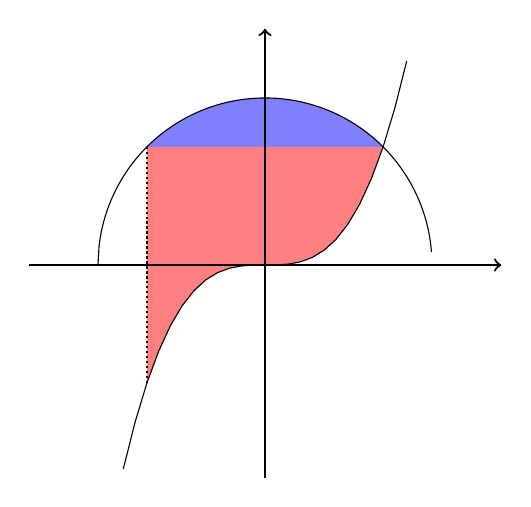
\begin{tikzpicture}[scale=1.5]
        \fill[blue!50!white, domain=-1:1, variable=\x]
            (-1,1) -- plot ({\x}, {sqrt(2-\x*\x)}) -- cycle;
        \fill[red!50!white, domain=-1:1, variable=\x]
            (-1,-1) -- plot ({\x}, {\x*\x*\x}) -- (-1, 1) -- cycle;
        \draw[black, domain={-sqrt(2)}:{sqrt(2)}, variable=\x, samples=300]
            plot ({\x}, {sqrt(2-\x*\x)});
        \draw[black, domain=-1.2:1.2, variable=\x]
            plot ({\x}, {\x*\x*\x});
        \draw[black, densely dotted, thick]
            (-1,-1) -- (-1,1);
        \draw[->, black, thick]
            (-2,0) -- (2,0);
        \draw[->, black, thick]
            (0,-1.8) -- (0,2);
    \end{tikzpicture}\par}

    The blue region is given by $1\leq y\leq\sqrt2$ and $-\sqrt{2-y^2}\leq x\leq\sqrt{2-y^2}$, and the red region is $-1\leq y\leq1$ and $-1\leq x\leq\sqrt[3]y$.
    So the integral is
    \[ \int_{-1}^1\int_{-1}^{\sqrt[3]y}f(x,y)\,dxdy + \int_{1}^{\sqrt2}\int_{-\sqrt{2-y^2}}^{\sqrt{2-y^2}}f(x,y)\,dxdy \]
\eblank

\bexerc
    Compute
    \[ \iint_D\frac1{\sqrt{x^2+y^2}}\,dxdy \]
    where $D=\set{(x,y)\in\bR^2}[\parens{x-\frac12}^2+\parens{y-\frac12}^2\leq\frac12]$.
\eexerc

\bblank
    Note that
    \[ \parens{x-\frac12}^2+\parens{y-\frac12}^2 = x^2 + y^2 - x - y + \frac12 \]
    So $(x,y)\in D$ if and only if $x^2+y^2-x-y\leq0$.
    Let us transform to polar coordinates, this means that we're in the domain if and only if
    \[ r^2 \leq r(\cos\theta+\sin\theta) \iff r\leq\cos\theta+\sin\theta \]
    And $0\leq\cos\theta+\sin\theta$ if and only if $-\frac\pi4\leq\theta\leq\frac{3\pi}4$ so the integral is
    \[ \int_{-\frac\pi4}^{\frac{3\pi}4}\int_0^{\cos\theta+\sin\theta}1\,drd\theta = \int_{-\frac\pi4}^{\frac{3\pi}4}\cos\theta+\sin\theta\,d\theta \]
    This is equal to $2\sqrt2$.
\eblank

\bexerc
    Compute
    \[ \iint_D e^{\frac{x-y}{x+y}}\,dxdy \]
    where $D=\set{1\leq x+y\leq 2, x\geq0, y\geq0}$.
\eexerc

\bblank
    We transform $u=x+y$ and $v=x-y$, or $x=\frac{u+v}2$ and $y=\frac{u-v}2$.
    Thus the Jacobian is
    \[ \abs{{\def\arraystretch{1.3}\begin{vmatrix}\frac12 & \hphantom{-}\frac12 \\ \frac12 & -\frac12\end{vmatrix}}} = \frac12 \]
    And the domain becomes $1\leq u\leq 2$, $u+v\geq0$, and $u-v\geq0$, so $\set{1\leq u\leq2, -u\leq v\leq u}$, so:
    \[ \frac12\int_1^2\int_{-u}^u e^{\frac vu}\,dvdu = \frac12\int_1^2 u\parens{e-\frac1e}\,dy = \frac34\parens{e-\frac1e} \]
\eblank

\bexerc
    Compute
    \[ \iiint_D(yz+zx)\,dxdydz \]
    where $D$ is the domain contained within the first octant, $x=0$, $z=0$, $y=x$, $x^2+y^2+z^2=R^2$.
\eexerc

\bblank
    Here
    \[ D = \set{z\geq0, 0\leq y\leq x, x^2+y^2+z^2\leq R^2} \]
    Let us use spherical coordinates $(\rho, \phi, \theta)$ where
    \[ x = \rho\sin\phi\cos\theta,\quad y=\rho\sin\phi\sin\theta,\quad z=\rho\cos\phi \]
    subject to
    \[ \rho\geq0,\quad 0\leq\phi\leq\pi,\quad -\pi\leq\theta\leq\pi \]
    The Jacobian is well-known $\phi^2\sin\phi$.
    And the domain requires $\phi\leq R$, $\cos\phi\geq0$ meaning $0\leq\phi\leq\frac\pi2$.
    This means that $\sin\phi\geq0$, and the domain requires $0\leq\sin\phi\cos\theta\leq\sin\phi\sin\theta$, so $0\leq\cos\theta\leq\sin\theta$.
    $\cos\theta\geq0$ so $-\frac\pi2\leq\theta\leq\frac\pi2$ and $\sin\theta\geq0$ so $0\leq\theta\leq\frac\pi2$ and finally $\tan\theta\geq1$ so $\frac\pi4\leq\theta\leq\frac\pi2$.

    And the integrand is
    \[ \rho^2\cos\phi\sin\phi(\cos\theta+\sin\theta)\rho^2\sin\phi = \rho^4\cos\phi\sin^2\phi(\cos\theta+\sin\theta) \]
    So the integral is
    \[ \int_0^R\int_0^{\frac\pi2}\int_{\frac\pi4}^{\frac\pi2}\rho^4\cos\phi\sin^2\phi(\cos\theta+\sin\theta)\,d\theta d\phi d\rho \]
    This is simply the product
    \[ \int_0^R\rho^4\,d\rho\cdot\int_0^{\frac\pi2}\sin^2\phi\cos\phi\,d\phi\cdot\int_{\frac\pi4}^{\frac\pi2}\cos\theta+\sin\theta\,d\theta \]
    The first integral is equal to $\frac{R^5}5$, and the last integral is
    \[ \sin\theta - \cos\theta\Bigl|_{\frac\pi4}^{\frac\pi2} = 1 \]
    The second integral is
    \[ \int_0^{\frac\pi2}\bigl(\sin\phi\bigr)^2\,d\bigl(\sin\phi\bigr) = \frac13 \]
    So the integral is equal to
    \[ \frac{R^5}{15} \]

\eblank

\end{document}

